\documentclass{article}
\usepackage[utf8]{inputenc}

\title{Fall 2020 CS4641 Homework 2}
\author{Aman Singh}

\usepackage{natbib}
\usepackage{graphicx}
\usepackage{amsmath}
\usepackage{amssymb}
\usepackage{enumitem}
\usepackage{hyperref}
\usepackage{slashbox}

\makeatletter
\renewcommand*\env@matrix[1][*\c@MaxMatrixCols c]{%
  \hskip -\arraycolsep
  \let\@ifnextchar\new@ifnextchar
  \array{#1}}
\makeatother

\hypersetup{
    colorlinks=true,
    linkcolor=blue,
    filecolor=magenta,      
    urlcolor=cyan,
    pdftitle={Sharelatex Example},
    bookmarks=true,
    pdfpagemode=FullScreen,
}
\begin{document}
\maketitle

\section{1.4 COVID19 Clustering}
\begin{verbatim}
    *** Expected Answer ***
==x==
[[ 1.62434536 -0.61175641]
 [-0.52817175 -1.07296862]]
==y==
[[ 0.86540763 -2.3015387 ]
 [ 1.74481176 -0.7612069 ]
 [ 0.3190391  -0.24937038]]
==dist==
[[1.85239052 0.19195729 1.35467638]
 [1.85780729 2.29426447 1.18155842]]

*** My Answer ***
==x==
[[ 1.62434536 -0.61175641]
 [-0.52817175 -1.07296862]]
==y==
[[ 0.86540763 -2.3015387 ]
 [ 1.74481176 -0.7612069 ]
 [ 0.3190391  -0.24937038]]
==dist==
[[1.85239052 0.19195729 1.35467638]
 [1.85780729 2.29426447 1.18155842]]
\end{verbatim}
\begin{verbatim}
    Cluster 1: Average confirmed: 18495.95, Average Deathtoll: 1260.88.
Total number of countries in Cluster 1: 186
Afghanistan   Albania   Algeria   Andorra   Angola   Antigua and Barbuda   Argentina   Armenia   Australia   Austria   


Cluster 2: Average confirmed: 1551853.00, Average Deathtoll: 93439.00.
Total number of countries in Cluster 2: 1
US   
\end{verbatim}
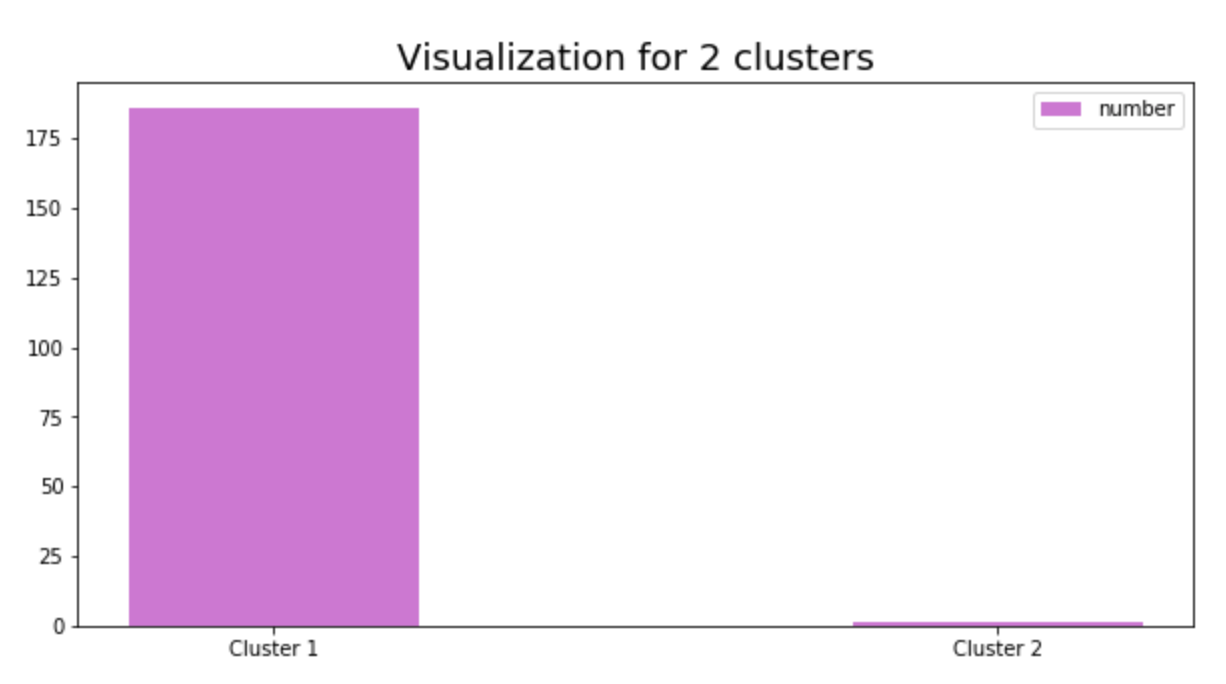
\includegraphics[scale=0.75]{cluster_graph.png}
\begin{verbatim}
    Cluster 1: Average confirmed: 238005.43, Average Deathtoll: 21997.29.
Total number of countries in Cluster 1: 7
Brazil   France   Germany   Italy   Russia   Spain   United Kingdom   


Cluster 2: Average confirmed: 1551853.00, Average Deathtoll: 93439.00.
Total number of countries in Cluster 2: 1
US   


Cluster 3: Average confirmed: 38857.69, Average Deathtoll: 2196.06.
Total number of countries in Cluster 3: 16
Bangladesh   Belarus   Belgium   Chile   Ecuador   Ireland   Mexico   Netherlands   Pakistan   Portugal   


Cluster 4: Average confirmed: 3126.38, Average Deathtoll: 106.68.
Total number of countries in Cluster 4: 157
Afghanistan   Albania   Algeria   Andorra   Angola   Antigua and Barbuda   Argentina   Armenia   Australia   Austria   


Cluster 5: Average confirmed: 110274.17, Average Deathtoll: 4776.17.
Total number of countries in Cluster 5: 6
Canada   China   India   Iran   Peru   Turkey   
\end{verbatim}
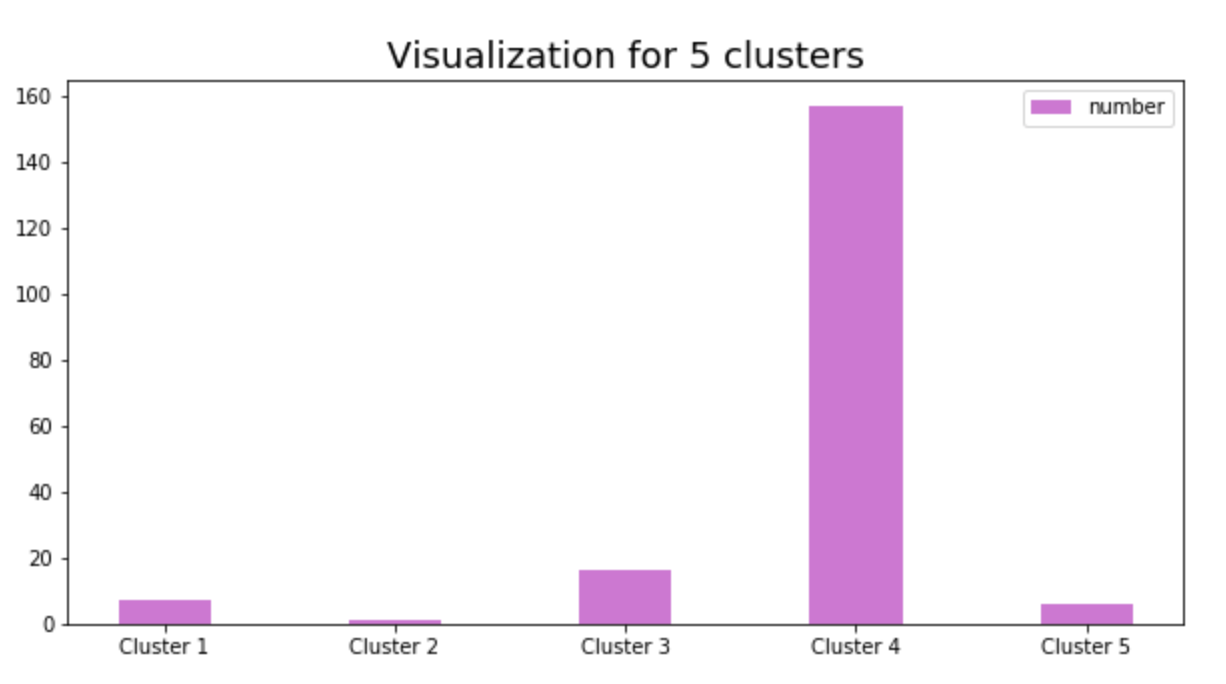
\includegraphics[scale=0.75]{cluster_graph2.png}\newline
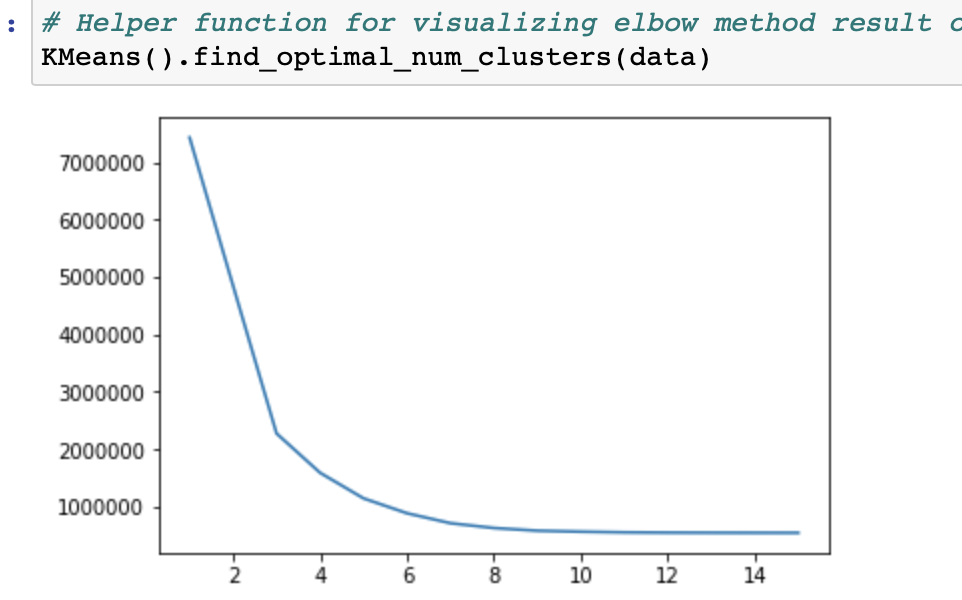
\includegraphics[scale=0.75]{matplotlib.png}
\begin{verbatim}
    array([7434367.7420582 , 4852386.66533115, 2276962.03134415,
       1592353.77568804, 1145999.12358172,  886437.16895716,
        712883.52615077,  628874.04067566,  581848.96712448,
        565261.31570247,  553220.81680461,  548550.30293357,
        546688.05497469,  545499.81498079,  545074.20034259])
\end{verbatim}
\begin{verbatim}
    Cluster 1: Average recovered: 2704795.29, Average confirmed: 4429822.62, Average Deathtoll: 227358.44.
Total number of countries in Cluster 1: 184
Afghanistan   Albania   Algeria   Andorra   Angola   Antigua and Barbuda   Argentina   Armenia   Australia   Austria   


Cluster 2: Average recovered: 114476468.33, Average confirmed: 242568774.00, Average Deathtoll: 9048283.00.
Total number of countries in Cluster 2: 3
Brazil   India   US   
\end{verbatim}
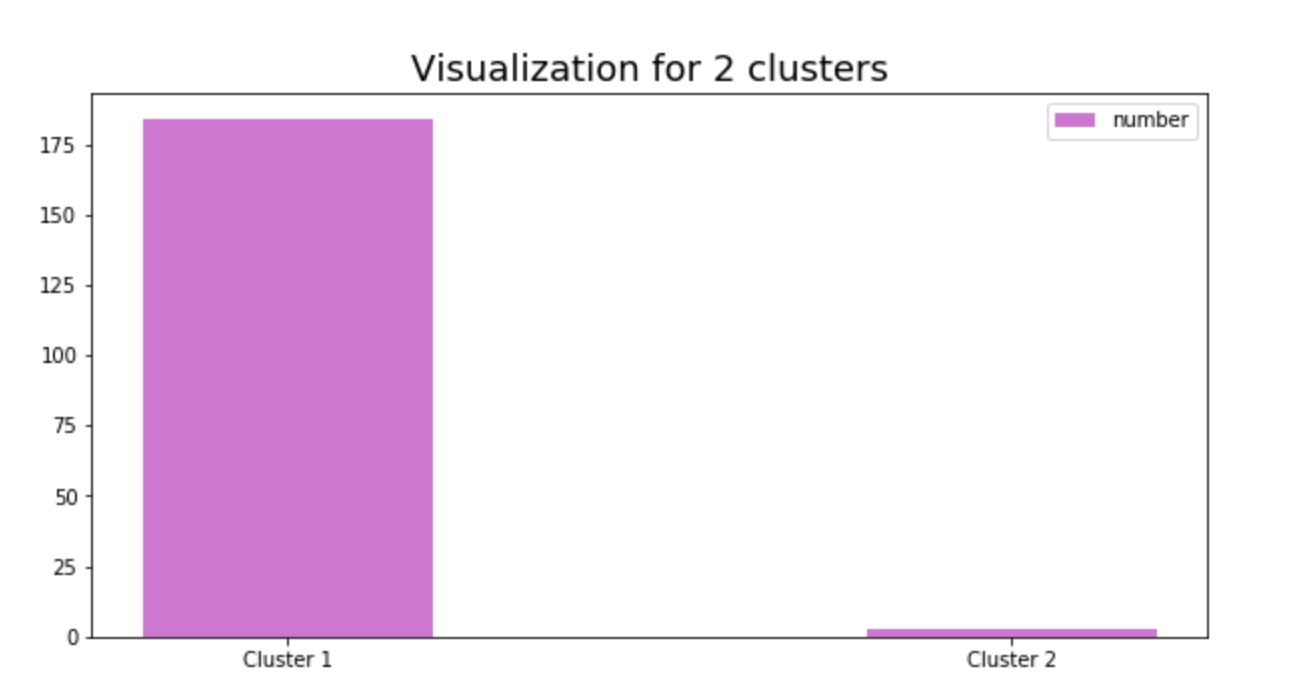
\includegraphics[scale=0.75]{cluster_graph3.png}
\begin{verbatim}
    Cluster 1: Average recovered: 67424447.00, Average confirmed: 101308266.00, Average Deathtoll: 1955657.50.
Total number of countries in Cluster 1: 2
India   Russia   


Cluster 2: Average recovered: 129005629.50, Average confirmed: 300667433.00, Average Deathtoll: 12187388.50.
Total number of countries in Cluster 2: 2
Brazil   US   


Cluster 3: Average recovered: 4132179.44, Average confirmed: 7527867.22, Average Deathtoll: 295142.63.
Total number of countries in Cluster 3: 27
Argentina   Bangladesh   Belarus   Belgium   Bolivia   Canada   Dominican Republic   Ecuador   Egypt   Indonesia   


Cluster 4: Average recovered: 424307.55, Average confirmed: 672968.22, Average Deathtoll: 17542.06.
Total number of countries in Cluster 4: 141
Afghanistan   Albania   Algeria   Andorra   Angola   Antigua and Barbuda   Armenia   Australia   Austria   Azerbaijan   


Cluster 5: Average recovered: 18457025.07, Average confirmed: 29380090.20, Average Deathtoll: 2016695.20.
Total number of countries in Cluster 5: 15
Chile   China   Colombia   France   Germany   Iran   Italy   Mexico   Pakistan   Peru   
\end{verbatim}
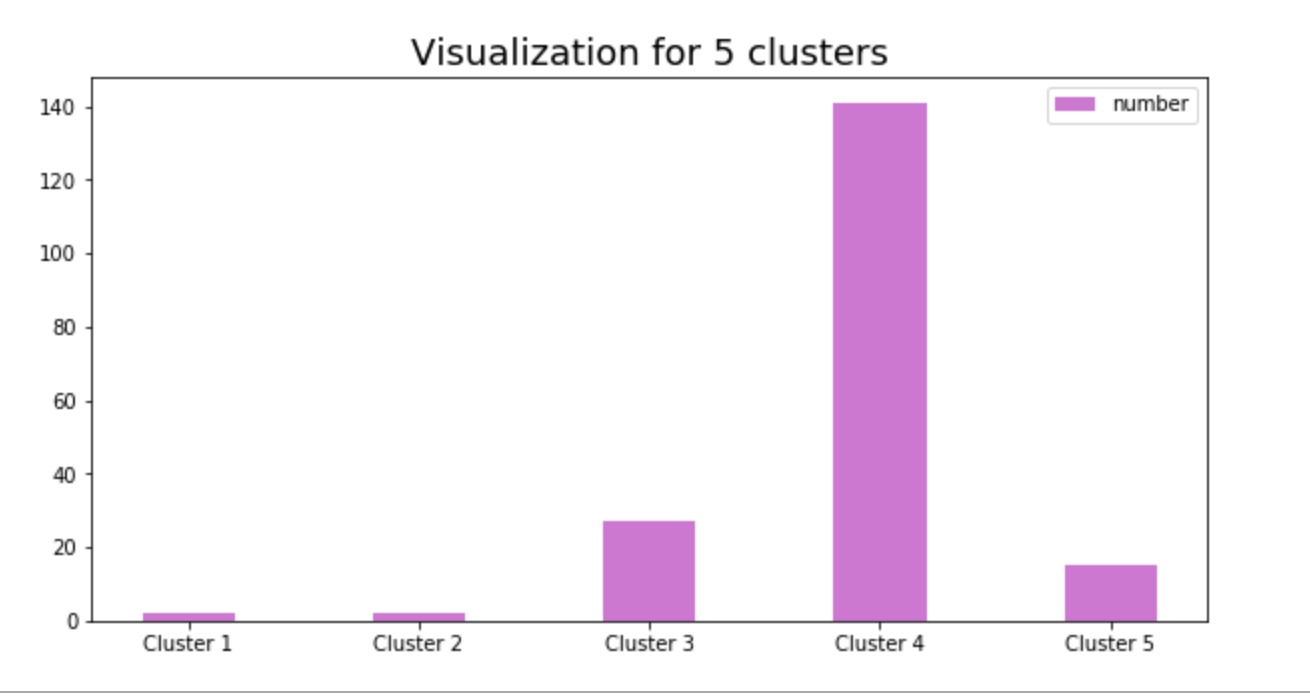
\includegraphics[scale=0.75]{cluster_graph4.png} \newline
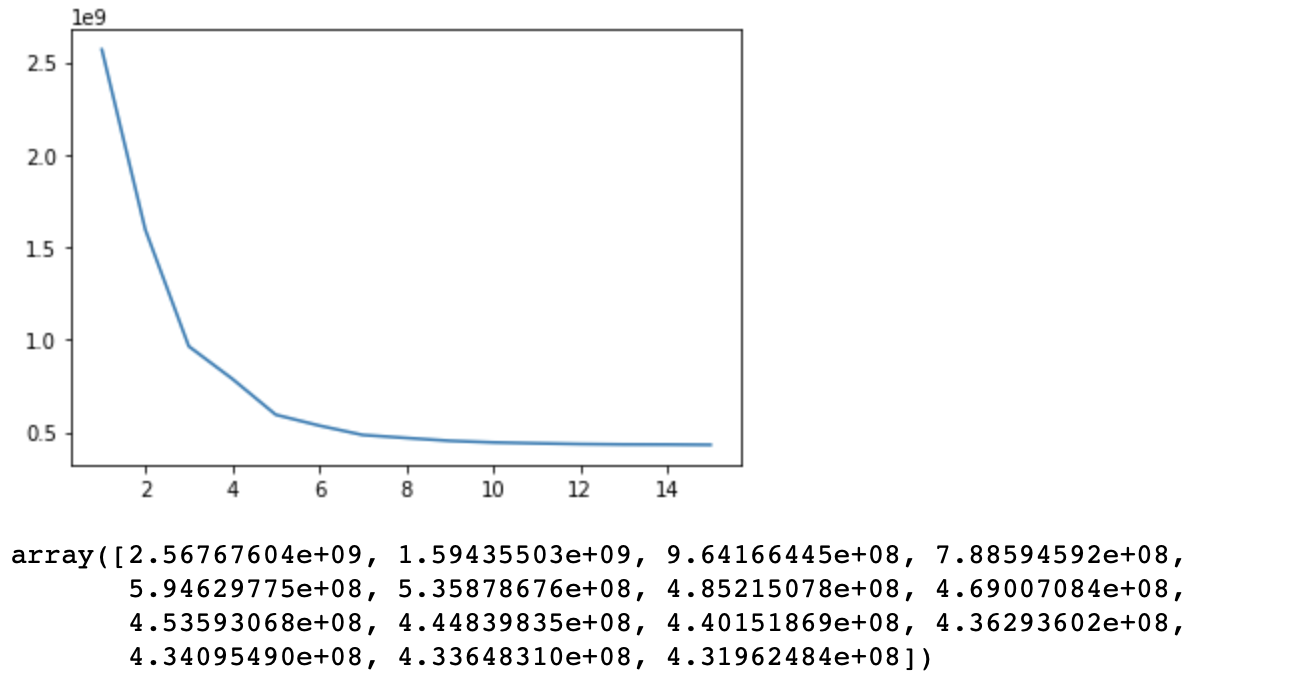
\includegraphics[scale=0.75]{matplotlib2.png}
\begin{verbatim}
    Cluster 1: Average confirmed: 196511.09, Average Deathtoll: 15622.18.
Total number of countries in Cluster 1: 11
Brazil   France   Germany   India   Iran   Italy   Peru   Russia   Spain   Turkey   


Cluster 2: Average confirmed: 1551853.00, Average Deathtoll: 93439.00.
Total number of countries in Cluster 2: 1
US   


Cluster 3: Average confirmed: 7306.43, Average Deathtoll: 358.17.
Total number of countries in Cluster 3: 175
Afghanistan   Albania   Algeria   Andorra   Angola   Antigua and Barbuda   Argentina   Armenia   Australia   Austria   
\end{verbatim}

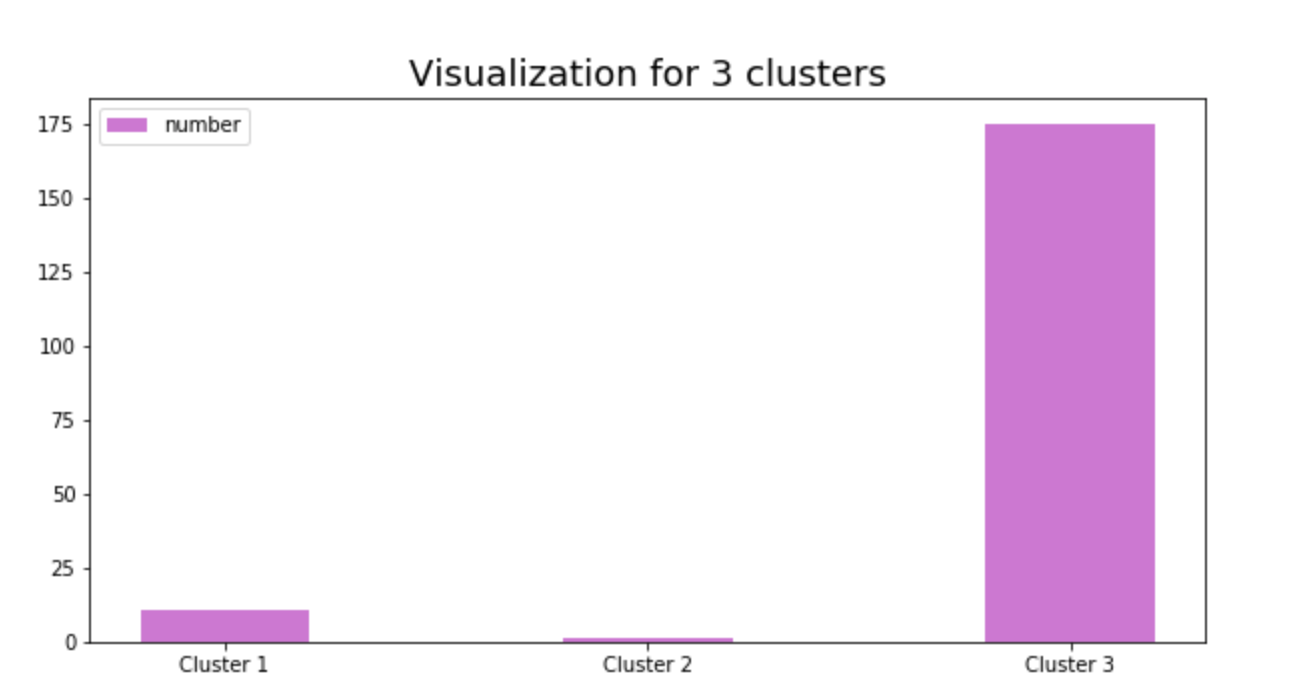
\includegraphics[scale=0.75]{cluster_graph5.png}
\begin{verbatim}
    Cluster 1: Average confirmed: 39135219.81, Average Deathtoll: 2083109.62.
Total number of countries in Cluster 1: 16
Chile   Colombia   France   Germany   India   Iran   Italy   Mexico   Pakistan   Peru   


Cluster 2: Average confirmed: 300667433.00, Average Deathtoll: 12187388.50.
Total number of countries in Cluster 2: 2
Brazil   US   


Cluster 3: Average confirmed: 1865652.67, Average Deathtoll: 66711.66.
Total number of countries in Cluster 3: 169
Afghanistan   Albania   Algeria   Andorra   Angola   Antigua and Barbuda   Argentina   Armenia   Australia   Austria   

\end{verbatim}
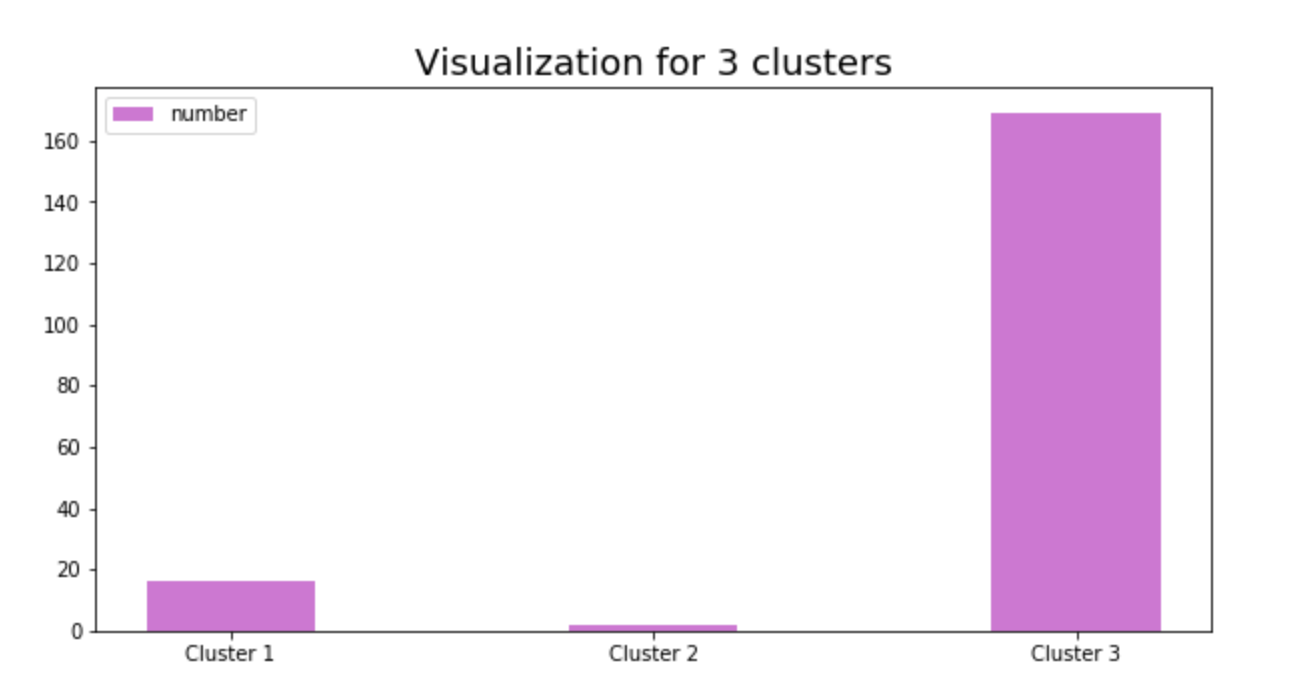
\includegraphics[scale=0.75]{cluster_graph6.png}

\section{B}
It seems like the data always has one cluster that is much bigger than the other
clusters combined, when using this algorithm. Assuming that this method is not flawed,
that means that there are certain groups of countries that control it similar to each other.
Of course, America is its own cluster because our handling of COVID-19 has been horrible.

\end{document}
